\chapter{Artificial Intellingence}

\label{chapter:AI}

The present chapter has the purpose of \textit{explaining} the database \textbf{interpolation} using a \textbf{machine learning model}. 

\section{Problem Framing}

The machine learning algorithm is based on a regression algorithm. 
The regression algorithm is based on a domain interpolation which does not include any aleatory variable.

This algorithm \textit{predicts} a \textbf{blade geometry} giving as input the \textbf{aerodynamic duty} and the \textbf{aerodynamic style}. 
The blades are parametrized the same way the database's blade are.

Figure~\ref{fig:MLstructure} is a representation of the machine learning structure.

\begin{figure}[!h]
    \newcommand\WIDTH{3cm}
\newcommand\HEIGHT{1.25cm}
\newcommand\Ydist{0.2cm}
\newcommand\XPOS{1cm}
\newcommand\TOTheight{6.2cm}
\newcommand\TOTwidth{4cm}
\newcommand\PTS{1.2pt}
\newcommand\SHADOWred{50}
\newcommand\SHADOWgreen{30}
\newcommand\SHADOWblue{20}

\newcommand\blockHeight{1.5cm}
\newcommand\blockWidth{4cm}

\centering

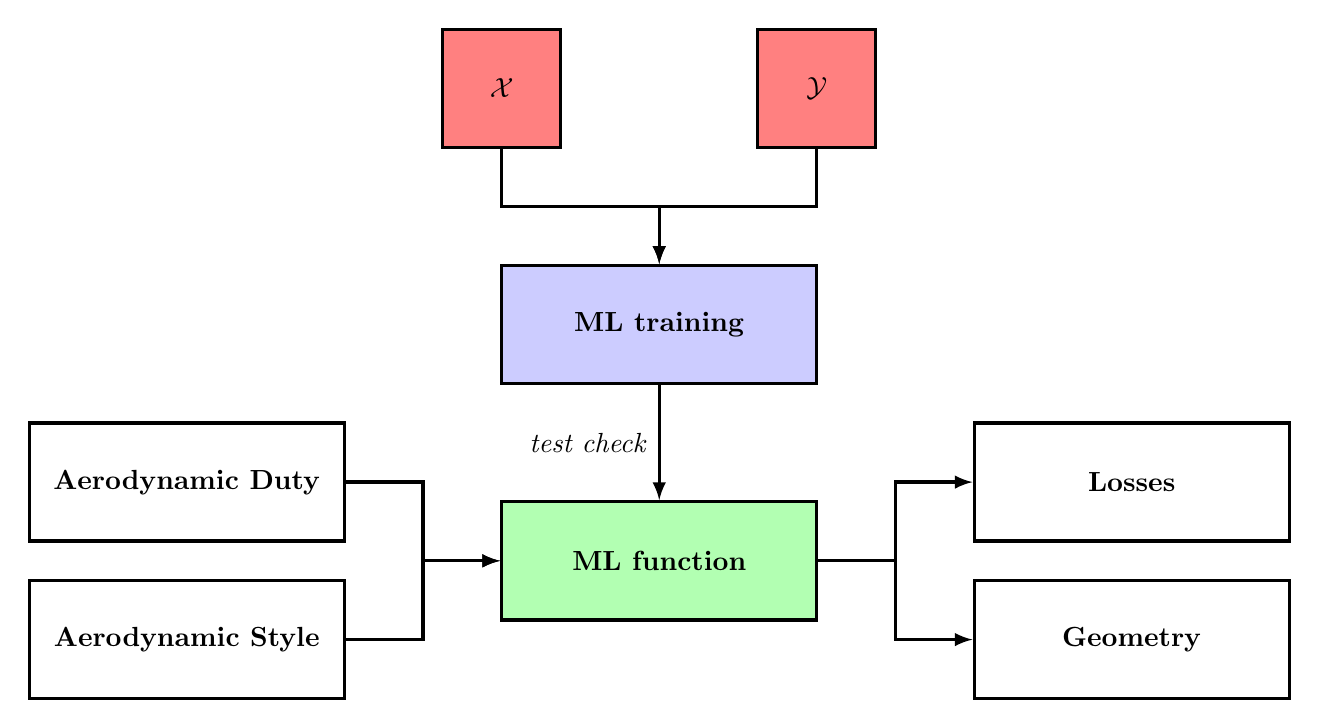
\begin{tikzpicture}
    
    \node[draw,
        rectangle,
        % rounded corners,
        line width = \PTS,
        minimum height = \blockHeight,
        minimum width = \blockWidth,
        fill = blue!\SHADOWblue,
    ] (AI) at (0, 0) {\textbf{ML training}};

    \node[draw,
        rectangle,
        % rounded corners,
        line width = \PTS,
        minimum height = \blockHeight,
        minimum width = \blockHeight,
        fill = red!\SHADOWred,
    ] (X) at (-2, 3) {$\mathcal{X}$};

    \node[draw,
        rectangle,
        % rounded corners,
        line width = \PTS,
        minimum height = \blockHeight,
        minimum width = \blockHeight,
        fill = red!\SHADOWred,
    ] (Y) at (2, 3) {$\mathcal{Y}$};

    \node[draw,
        rectangle,
        % rounded corners,
        line width = \PTS,
        minimum height = \blockHeight,
        minimum width = \blockWidth,
        fill = green!\SHADOWgreen,
    ] (func) at (0, -3) {\textbf{ML function}};
    
    \node[draw,
        rectangle,
        % rounded corners,
        line width = \PTS,
        minimum height = \blockHeight,
        minimum width = \blockWidth
    ] (inputDuty) at (-6, -2) {\textbf{Aerodynamic Duty}};

    \node[draw,
        rectangle,
        % rounded corners,
        line width = \PTS,
        minimum height = \blockHeight,
        minimum width = \blockWidth
    ] (inputStyle) at (-6, -4) {\textbf{Aerodynamic Style}};

    \node[draw,
        rectangle,
        % rounded corners,
        line width = \PTS,
        minimum height = \blockHeight,
        minimum width = \blockWidth
    ] (outputGeometry) at (6, -4) {\textbf{Geometry}};

    \node[draw,
        rectangle,
        % rounded corners,
        line width = \PTS,
        minimum height = \blockHeight,
        minimum width = \blockWidth
    ] (outputProperty) at (6, -2) {\textbf{Losses}};

    \coordinate[] (c1) at (-2, 1.5) {};
    \coordinate[] (c2) at (2,  1.5) {};
    \coordinate[] (c3) at (0,  1.5) {};
    \coordinate[] (c4) at (-3,  -2) {};
    \coordinate[] (c5) at (-3,  -4) {};
    \coordinate[] (c6) at (-3,  -3) {};
    \coordinate[] (c7) at (3,  -2) {};
    \coordinate[] (c8) at (3,  -4) {};
    \coordinate[] (c9) at (3,  -3) {};

    \draw[-latex, line width=\PTS] (X.south) -- (c1) -- (c3) to (AI.north);
    \draw[-latex, line width=\PTS] (Y.south) -- (c2) -- (c3) to (AI.north);
    \draw[-latex, line width=\PTS] (AI) -- node[anchor=east] {\textit{test check}} (func);
    \draw[-latex, line width=\PTS] (inputDuty.east)  -- (c4) -- (c6) to (func.west);
    \draw[-latex, line width=\PTS] (inputStyle.east) -- (c5) -- (c6) to (func.west);
    \draw[-latex, line width=\PTS] (func.east) -- (c9) -- (c7) to (outputProperty.west);
    \draw[-latex, line width=\PTS] (func.east) -- (c9) -- (c8) to (outputGeometry.west);

\end{tikzpicture}

    \caption{Machine learning model.}
    \label{fig:MLstructure}
\end{figure}

\section{Interpolation}

The regression starts with the definition of the domains of study:

\begin{itemize}
    \item $\mathcal{X}$ contains the aerodynamic style and aerodynamic duty properties. 
    $\mathcal{X} \in \mathbb{R}^{2787 \times 8}$: where $2787$ is the number of filtered blades and $8$ are the number of parameters for defining the aerodynamic style and the aerodynamic duty of the blade.
    The $\boldsymbol{x}$ vector is the general element of $\mathcal{X}$
    % which stores the aerodynamic style and the aerodynamic duty of the database point
    \item $\mathcal{Y}$ stores the camberline and Kulfan parameters for the description of the blade. 
    $\mathcal{Y} \in \mathbb{R}^{2787 \times 42}$: where $2787$ is the number of blades and $42$ is the number of parameters used for representing each blade - Kulfan parameters and pitch.
    The $\boldsymbol{y}$ vector is the general element of $\mathcal{Y}$
    % which stores the blade parametrization for the camberline, the pressure side and suction side of the blade
\end{itemize}

The machine learning algorithm has the goal to find an approximation of a mapping function, $\mathnormal{f}$, which relates the 
two domains, $\mathcal{X}$ and $\mathcal{Y}$. 

Ideally, the mapping function, $\mathnormal{f}$, defines Equation~(\ref{eqn:mapFunc}):

\begin{equation}
    \mathnormal{f}_{(\boldsymbol{x})} = \boldsymbol{y}
    \label{eqn:mapFunc}
\end{equation}

The machine learning algorithm has the role of computing $\hat{\mathnormal{f}}$ which is the numerical approximation of $\mathnormal{f}$.
The new function, $\hat{\mathnormal{f}}$, will define the following problem:

\begin{equation}
    \hat{\mathnormal{f}}_{(\boldsymbol{x})} \approx \boldsymbol{y}
    \label{eqn:mapFuncML}
\end{equation}

For the computation of $\hat{\mathnormal{f}}$, the $\mathcal{X}$ and $\mathcal{Y}$ domains are splitted into two sub-domains each. 
For the present work, a splitting factor of $30\%$ has been used after extensive tests over the many possible factors.
The splitting will then generate four sub-domains:

\begin{itemize}
    \item $\mathcal{X}$ domain: 
        \begin{itemize}
            \item training set: $\mathcal{X}_{*}$, made by $\boldsymbol{x}_{*}$ 
            \item test set: $\mathcal{X}_{**}$, made by $\boldsymbol{x}_{**}$
        \end{itemize}
    \item $\mathcal{Y}$ domain:
        \begin{itemize} 
            \item training set: $\mathcal{Y}_{*}$, made by $\boldsymbol{y}_{*}$
            \item test set: $\mathcal{Y}_{**}$, made by $\boldsymbol{y}_{**}$
        \end{itemize}
\end{itemize}

\subsection{Radial Basis Function}

Once introduced the main purpose of the machine learning algorithm, it is necessary to find a \textbf{suitable regression algorithm}
to interpolate the domain. In the present work, the radial basis functions~\cite{hensman2013gaussian} (RBF) are used as the kernel 
of the machine learning model. These functions are a very powerful tool for the interpolation of data. 
The overfitting problem is manageable and the model allows perfect interpolation of the training points, $(\boldsymbol{x}_{*}, \boldsymbol{y}_{*})$.

Equation~(\ref{eqn:RBF}) formulates the radial basis functions kernel:

\begin{align}
    d_j (\boldsymbol{x}) & = \lvert \boldsymbol{x} - \boldsymbol{x}^j_* \lvert \label{eqn:distance} \\
    \Phi_{j_{ ( \boldsymbol{x}, \ \boldsymbol{x}^j_*, \ c_j ) }} & = exp \big( -c^2_j \ d_j (\boldsymbol{x})^2 \big) \label{eqn:RBF} 
\end{align}

The kernel on its side relies on its length scale, $c_j$, and on the euclidean norm
between two points in the domain, $\boldsymbol{x}$ and $\boldsymbol{x}^{j}_*$, 
as presented in Equation~(\ref{eqn:distance}). 

From Equation~(\ref{eqn:RBF}) it is possible to understand that the higher the euclidean 
distance the lower the influence of a point $\boldsymbol{x}$ in the system. 
This is a very \textbf{powerful feature} because it decorrelates blades which define
aerodynamic duties and aerodynamic styles that are completely different.

At the same time, the usage of gaussian functions for the approximation of the domain
allows to \textbf{smooth out} $\hat{\mathnormal{f}}$. This feature is very important because it 
guarantees a smooth variation of the geometrical properties of the blade allowing a 
smooth change of the camberline and Kulfan parameters~\cite{duvenaud2014kernel}.
Figure~\ref{fig:RBF} shows the radial basis functions with a fixed length scale.

\begin{figure}[H]
    \centering
    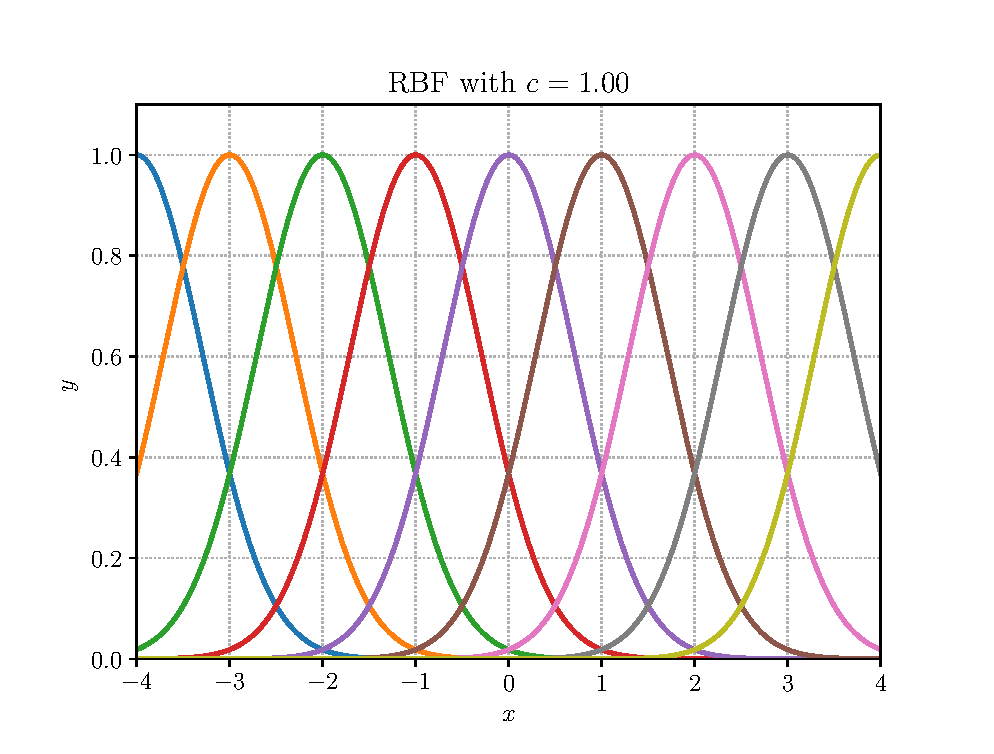
\includegraphics[width=0.5\textwidth]{./pyFigure/figures/RBF.eps}
    \caption{Radial Basis Functions.}
    \label{fig:RBF}
\end{figure}

\subsection{Training \& Testing}

Having set the fundamentals of the machine learning algorithm, it is necessary to construct the system for the 
computation of $\hat{\mathnormal{f}}$. The problem is defined by a linear system of equations.
These equations are a linear combinations of radial basis functions, Equation~(\ref{eqn:RBF}), which are 
weighted by parameters which take the name of \textit{weights}. These weights have the role to 
\textit{properly} fit the radial basis functions into the database.
The following set of equations represent the problem: 

\begin{align}
    \mathnormal{f} \approx \hat{\mathnormal{f}} & = \boldsymbol{\Phi}_{(\boldsymbol{x})} \cdot \boldsymbol{w} \\
    \boldsymbol{y} \approx \hat{\mathnormal{f}}_{(\boldsymbol{x}, \boldsymbol{w})} & = \boldsymbol{\Phi}_{(\boldsymbol{x})} \cdot \boldsymbol{w} \\ 
    \boldsymbol{\Phi}_{(\boldsymbol{x})} & = 
    \begin{bmatrix}
        \lvert &  & \lvert \\ 
        \Phi_{0_{ ( \boldsymbol{x}, \ \boldsymbol{c}_0 ) } } & ... & \Phi_{n_{ ( \boldsymbol{x}, \ \boldsymbol{c}_{m_*} ) } } \\
        \lvert &  & \lvert 
    \end{bmatrix}
    \label{eqn:phi}
\end{align}

Once the linear system is set, it is necessary to define a way for computing $\boldsymbol{w}$.
The problem will reduce to a minimization problem. The problem is characterized by the search of
the weight $\boldsymbol{w}$ such that a cost function is reduced to its minimum. The problem is 
represented by Equation~(\ref{eqn:MLminimization}):

\begin{equation}
    min \Bigg( J_{(\boldsymbol{x_*})} = \frac{1}{m_*} \sum^{m_* - 1}_{j = 0} \big( \hat{\mathnormal{f}}_{ (\boldsymbol{x}^{j}_{\boldsymbol{*}}, \boldsymbol{w})} - \boldsymbol{y}^{j}_{\boldsymbol{*}}\big)^2 \Bigg)
    \label{eqn:MLminimization}
\end{equation}

For example, the matricial form for the $\gamma$ degree of freedom will be written as:

\begin{equation}
    \begin{bmatrix}
        \gamma^0     \\
        % \gamma^2     \\
        \vdots       \\
        \gamma^{m_* - 1} \\
        \gamma^{m_*} \\
        % \chi_1^{1}   \\
        % % \chi_1^{2}   \\
        % \vdots       \\ 
        % \chi_1^{m_*} \\
        % \chi_2^{1}   \\
        % % \chi_2^{2}   \\
        % \vdots       \\ 
        % \chi_2^{m_*} \\
        % A_0^{1}      \\
        % % A_0^{2}      \\
        % \vdots       \\ 
        % A_0^{m_*}    \\
        % \vdots       \\ 
        % \beta^{1}    \\
        % % \beta^{2}    \\
        % \vdots       \\ 
        % \beta^{m_*}  \\
        % pitch^{1}    \\
        % % pitch^{2}    \\
        % \vdots       \\ 
        % pitch^{m_*}  
    \end{bmatrix} 
    = 
    \begin{bmatrix}
        % \Phi_{0_{(\boldsymbol{x}^{0}_{*}, c_0)}} & \Phi_{1_{(\boldsymbol{x}^{0}_{*}, c_1)}} & \ldots & \Phi_{{m_{*} - 1}_{( \boldsymbol{x}^{0}_{*}, c_{m_{*} - 1})}} & \Phi_{{m_{*}}_{( \boldsymbol{x}^{0}_{*}, c_{m_{*}})}} \\
        % \Phi_{0_{(\boldsymbol{x}^{1}_{*}, c_0)}} & \Phi_{1_{(\boldsymbol{x}^{1}_{*}, c_1)}} & \ldots & \Phi_{{m_{*} - 1}_{( \boldsymbol{x}^{1}_{*}, c_{m_{*} - 1})}} & \Phi_{{m_{*}}_{( \boldsymbol{x}^{1}_{*}, c_{m_{*}})}} \\
        % \vdots & \vdots & \ddots & \vdots & \vdots \\
        % \Phi_{0_{(\boldsymbol{x}^{m_{*} - 1}_{*}, c_0)}} & \Phi_{1_{(\boldsymbol{x}^{m_{*} - 1}_{*}, c_1)}} & \ldots & \Phi_{{m_{*} - 1}_{( \boldsymbol{x}^{m_{*} - 1}_{*}, c_{m_{*} - 1})}} & \Phi_{{m_{*}}_{( \boldsymbol{x}^{m_{*} - 1}_{*}, c_{m_{*}})}} \\
        % \Phi_{0_{(\boldsymbol{x}^{m_{*}}_{*}, c_0)}}     & \Phi_{1_{(\boldsymbol{x}^{m_{*}}_{*}, c_1)}}     & \ldots & \Phi_{{m_{*} - 1}_{( \boldsymbol{x}^{m_{*}}_{*}, c_{m_{*} - 1})}}     & \Phi_{{m_{*}}_{( \boldsymbol{x}^{m_{*}}_{*}, c_{m_{*}})}}  
        \Phi_{0_{(\boldsymbol{x}^{0}_{*}, c_0)}} & \ldots & \Phi_{{m_{*} - 1}_{( \boldsymbol{x}^{0}_{*}, c_{m_{*} - 1})}} & \Phi_{{m_{*}}_{( \boldsymbol{x}^{0}_{*}, c_{m_{*}})}} \\
        \vdots & \ddots & \vdots & \vdots \\
        \Phi_{0_{(\boldsymbol{x}^{m_{*} - 1}_{*}, c_0)}} & \ldots & \Phi_{{m_{*} - 1}_{( \boldsymbol{x}^{m_{*} - 1}_{*}, c_{m_{*} - 1})}} & \Phi_{{m_{*}}_{( \boldsymbol{x}^{m_{*} - 1}_{*}, c_{m_{*}})}} \\
        \Phi_{0_{(\boldsymbol{x}^{m_{*}}_{*}, c_0)}}     & \ldots & \Phi_{{m_{*} - 1}_{( \boldsymbol{x}^{m_{*}}_{*}, c_{m_{*} - 1})}}     & \Phi_{{m_{*}}_{( \boldsymbol{x}^{m_{*}}_{*}, c_{m_{*}})}}  
    \end{bmatrix}_{\gamma}
    \cdot 
    \begin{bmatrix}
        w^0 \\ 
        % w^1 \\ 
        \vdots \\
        w^{m_* - 1} \\  
        w^{m_*}
    \end{bmatrix}_{\gamma}
    \label{eqn:MLmatricial}
\end{equation}

Equation~(\ref{eqn:MLmatricial}) shows a piece of the minimization problem in Equation~(\ref{eqn:MLminimization}). In this case the left hand side of the equation
shows a part of the $\boldsymbol{y_{*}}$ vector which correspond to the $\gamma$ optimization problem. The whole system is a concatenation of problems spanning 
all the Kulfan's parameters and the pitch. The matrix in Equation~(\ref{eqn:MLmatricial}) is a more detailed form of Equation~(\ref{eqn:phi}). The right hand side of 
Equation~(\ref{eqn:MLmatricial}) takes the $\gamma$ subscript: this to indicate that the elements are referred only to the $\gamma$ degree of freedom.

The optimization problem is solved by an iterative algorithm which finds the optimum solution, $\boldsymbol{w}$.
The optimization is conducted over the \textbf{training set}, $(\mathcal{X}_{*}, \mathcal{Y}_{*})$. 

Once $\boldsymbol{w}$ is computed, it is necessary to understand the \textit{quality} of the weights. 
This test is done using the \textbf{test set}, $(\mathcal{X}_{**}, \mathcal{Y}_{**})$ following Equation~(\ref{eqn:MLtest}):

\begin{equation}
    J_{(\boldsymbol{x_{**}})} = \frac{1}{m_{**}} \sum^{m_{**} - 1}_{j = 0} \big( \hat{\mathnormal{f}}_{ (\boldsymbol{x}^{j}_{\boldsymbol{**}}, \boldsymbol{w})} - \boldsymbol{y}^{j}_{\boldsymbol{**}}\big)^2 
    \label{eqn:MLtest}
\end{equation}

\subsection{Sckit-Learn}

The machine learning analysis of the system has been done using a robust and consolidated library: \textbf{Sckit-Learn}.

Listing~\ref{listing:dataPrep} represents the commands for the normalization of the whole database. In terms of 
operativity and interpolation errors, it is common use to normalize data in $[0, 1]$ interval.

\lstinputlisting[style=customPy, firstline=1, lastline=12, caption=Data preprocessing, label=listing:dataPrep]{./code/ML.txt}

Having preprocessed the data, it is necessary to split the normalized data into the training and test sets. 
Once the entries are randomly splitted, the RBF kernel is initialized for the usage in the interpolation algorithm.
The final step for the interpolation of the database consists into the minimization of the $J$ functional 
which computes the $\boldsymbol{w}$ vector. 

Listing~\ref{listing:RBF} represents all the above steps. 

\lstinputlisting[style=customPy, firstline=14, lastline=26, caption=RBF interpolation, label=listing:RBF]{./code/ML.txt}

Having optimized the radial basis function network, it is necessary to understand its properties; 
a test over the network is done using the test set. 

Listing~\ref{listing:test} computes the score of the interpolated network.

\lstinputlisting[style=customPy, firstline=36, caption=RBF scoring, label=listing:test]{./code/ML.txt}

The test scores the computed function, $\hat{\mathnormal{f}}$. 
The score gives an idea of how well the model fits the data in terms of explained variance.

The test scores a $3\%$ error. For the present work, the $\hat{\mathnormal{f}}$ computed satisfies 
the projects requirements. As result, $\hat{\mathnormal{f}}$ approximates the blade geometry given as 
inputs the aerodynamic style and the aerodynamic duty.

\subsection{Tuning}

Tuning the \textbf{hyperparameters} for a RBF kernel is an important step to achieve \textit{optimal performance}. 
The key hyperparameters to focus for the RBF network are:

\begin{itemize}
    \item Length Scale ($l$): This hyperparameter controls the \textit{smoothness} of the RBF kernel. A \textbf{smaller} length scale leads to a more \textbf{wiggly} and \textbf{flexible} kernel, while a \textbf{larger} length scale makes it \textbf{smoother}. 
    \item $\alpha$: This parameter determines the \textbf{regularization strength} of the model. It helps to \textbf{prevent overfitting} and stabilize the computations. A \textbf{larger} $\alpha$ places stronger emphasis on \textbf{noise reduction}.
\end{itemize}

The tuning has been done using a trial and error approach over the RBF lenght scale and the regularization parameter used by the regressor. 
The tuning has given:

\begin{itemize}
    \item $l = 0.1$ 
    \item $\alpha = 1 \cdot 10^{-3}$ 
\end{itemize}

Different parameters have been tested but they generated unacceptable errors at the boundaries of the domain of study due to the RBF properties. 
The gaussian functions do not show good accuracy at the boundaries because of the poor extrapolation properties of the method in that region of the domain.

\section{Results and Accuracy}

% In this section there will be shown the blade geometry extrapolation and load testing using the computed $\hat{\mathnormal{f}}$.
This section presents the extrapolation of the blade geometry and the load testing using the computed $\hat{\mathnormal{f}}$.

\begin{figure}[H]
    \centering 
    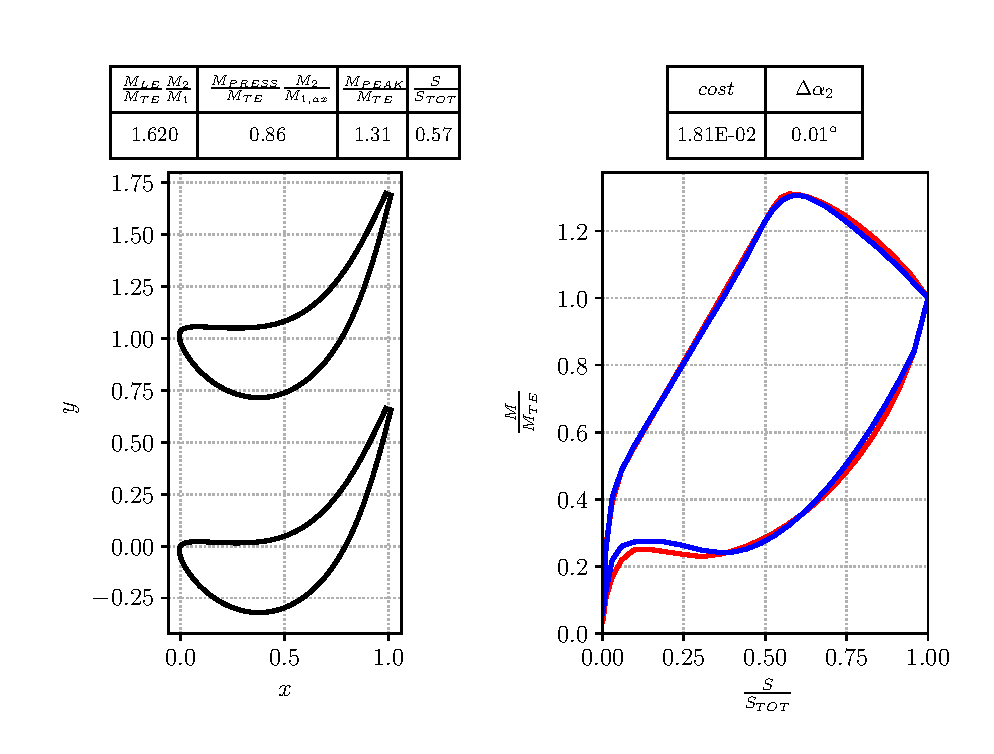
\includegraphics[scale=\scaleBlade]{./images/blade--3404-7015-57.eps}
    \caption{Blade generated by $\hat{\mathnormal{f}}$ with $\alpha_1 = -34.04^{\circ}$, $\alpha_2 = 70.15^{\circ}$ and $M_2 = 0.57$.}
    \label{fig:bladeML1}
\end{figure}

% Figure~\ref{fig:bladeML1} shows a blade computed from $\hat{\mathnormal{f}}$. This blade shows a $1.8\%$ error over the loading distribution
% and an error over the exit angle of $0.01^{\circ}$. The aerodynamic duty and aerodynamic style of the blade are away from 
% the $\mathcal{X}$ dataset entries.

In Figure~\ref{fig:bladeML1}, a blade computed from $\hat{\mathnormal{f}}$ is shown. This blade exhibits a $1.8\%$ error 
in the loading distribution and an error of $0.01^{\circ}$ in the exit angle. The aerodynamic duty and style of the 
blade differ from the entries in the $\mathcal{X}$ dataset.

Figure~\ref{fig:bladeML2} shows a blade which is considered acceptable for the design study of a section.

\begin{figure}[H]
    \centering 
    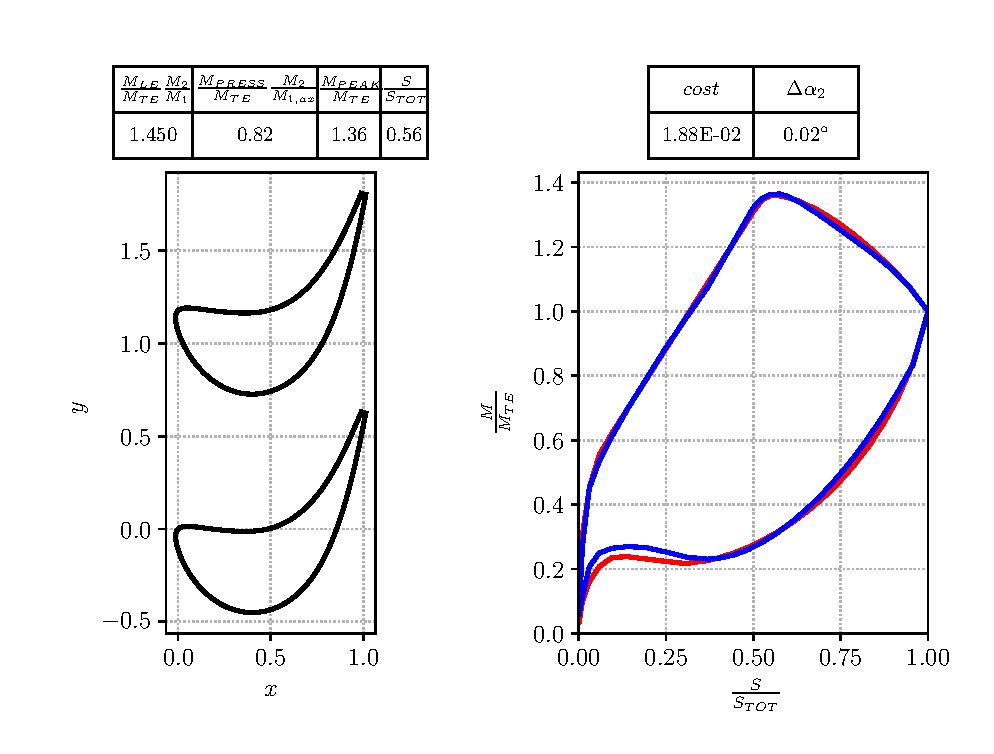
\includegraphics[scale=\scaleBlade]{./images/blade--4467-7211-41.eps}
    \caption{Blade generated by $\hat{\mathnormal{f}}$ with $\alpha_1 = -44.67^{\circ}$, $\alpha_2 = 72.11^{\circ}$ and $M_2 = 0.41$.}
    \label{fig:bladeML2}
\end{figure}

% Figure~\ref{fig:bladeML3} shows the lack of agreement with the target load because the limits of the 
% machine learning model based on the datasets of study, $(\mathcal{X}, \mathcal{Y})$.

Figure~\ref{fig:bladeML3} illustrates the discrepancy between the generated blade and the target load due to the limitations of the machine learning model based on the study datasets $(\mathcal{X}, \mathcal{Y})$.

\begin{figure}[H]
    \centering 
    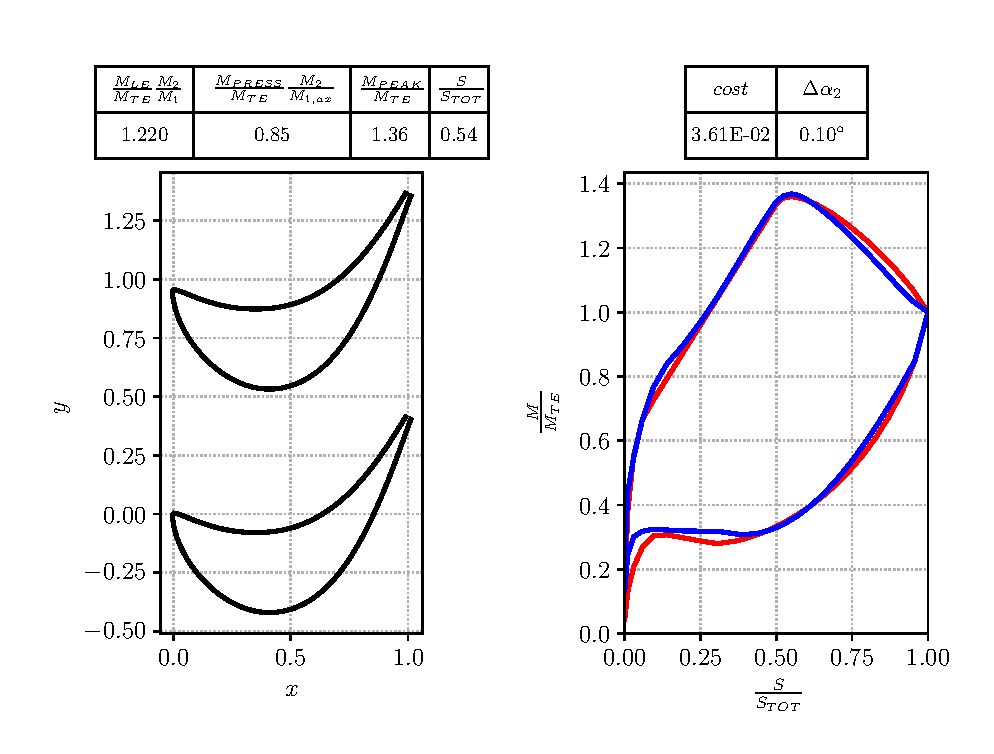
\includegraphics[scale=\scaleBlade]{./images/blade--4916-6516-67.eps}
    \caption{Blade generated by $\hat{\mathnormal{f}}$ with $\alpha_1 = -49.16^{\circ}$, $\alpha_2 = 65.16^{\circ}$ and $M_2 = 0.67$.}
    \label{fig:bladeML3}
\end{figure}

% Figure~\ref{fig:bladeML4} shows the same error behavior of Figure~\ref{fig:bladeML3}. After an extensive analysis of the 
% computed $\hat{\mathnormal{f}}$ function, the error \textbf{in the whole interpolated domain of study} remains under $4\%$,
% the exit angle error, $\Delta \alpha_2$, remains below $0.5^{\circ}$. These thresholds are considered acceptable 
% for a first alaysis of a blade using a fast design tool.

Figure~\ref{fig:bladeML4} demonstrates the same error pattern as seen in Figure~\ref{fig:bladeML3}. 
After an extensive analysis of the computed $\hat{\mathnormal{f}}$ function, the error throughout the entire interpolated domain of study 
remains under $4\%$, while the exit angle error ($\Delta \alpha_2$) remains below $0.5^{\circ}$. These thresholds are considered 
acceptable for an initial analysis of a blade using a rapid design tool.

\begin{figure}[H]
    \centering 
    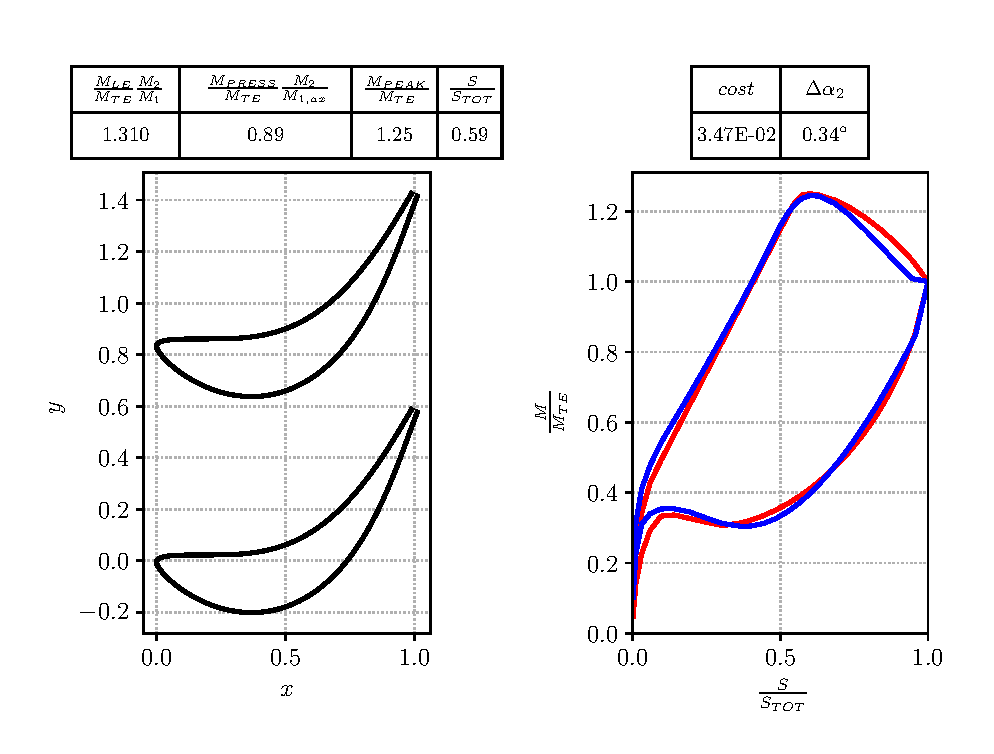
\includegraphics[scale=\scaleBlade]{./images/blade--2007-6516-60.eps}
    \caption{Blade generated by $\hat{\mathnormal{f}}$ with $\alpha_1 = -20.07^{\circ}$, $\alpha_2 = 65.16^{\circ}$ and $M_2 = 0.60$.}
    \label{fig:bladeML4}
\end{figure}
 